\chapter{Evaluating the MISR simulator using independently retrieved hydrometeor profiles from active sensors}\label{misr_chapter}

The goal of the instrument simulator approach is to remove ambiguities in comparisons between models and observations such that remaining differences between the observed and simulated cloud properties can be interpreted unambiguously as model errors. However, the simulators themselves have seen little critical evaluation. \cite{mace_et_al_2011}, hereafter M2011, performed an evaluation of the ISCCP simulator using thermodynamic and cloud property profiles derived from data collected at the Atmospheric Radiation Measurement Program \citep[ARM;][]{ackerman_and_stokes_2003} Southern Great Plains (SGP) ground-based observing site located near Lamont, Oklahoma. In their analysis, M2011 compare ARM radar-and-lidar derived cloud properties directly to those retrieved from ISCCP to first assess the biases in the ISCCP retrieval relative to the ARM-derived cloud properties. They then apply the ISCCP simulator to the ARM-derived profiles of cloud extinction and compare the ISCCP-simulated cloud properties to ISCCP retrievals. They find that the simulator accounts for much of the bias in the ISCCP cloud top pressure ($p_c$) retrieval; that is, the ISCCP-simulated $p_c$ retrieval compares well with the actual ISCCP retrieval. However, mid-level cloud remained a problem with significantly less mid-level cloud in the simulated retrievals than in the ISCCP retrievals (6\% relative to the total number of profiles, or equivalently, 23\% relative to the amount of simulated mid-level cloud), suggesting that the simulator does not completely compensate for the well-known tendency of ISCCP retrievals to overestimate the amount of mid-level clouds \citep[e.g.,]{marchand_et_al_2010}. More problematically, M2011 found large differences in optical depth between ISCCP and ARM retrievals. M2011 suggest this may be due to a combination of sub-pixel variability in the clouds and limitations associated with the 1D radiative transfer used in the ISCCP retrievals. The simulators do not current correct for any optical depth biases, and the potential exists for large biases in the comparisons for cases involving small, heterogeneous broken clouds where 3D effects become important. This topic is discussed in more detail later in this chapter, as it also affects the evaluation of the MISR simulator presented here.

The analysis by M2011 provides the only critical evaluation of the simulators documented in the available literature. The lack of verification of the simulators severely undermines their credibility for use in the evaluation of climate models. The goal of this chapter is to perform a similar analysis to M2011 for the MISR simulator. Conceptually similar to the ISCCP simulator, the MISR simulator produces histograms of cloud optical depth and cloud top height. While the optical depth retrievals are similar, the MISR cloud top height is based on a geometric stereo-imaging technique that has different strengths and weakness than ISCCP. In particular, MISR provides more accurate retrievals of cloud top height for low-level and mid-level clouds, more reliable discrimination of mid-level clouds from other clouds, and is insensitive to the instrument calibration making the data well suited for examining variability on seasonal or longer time scales, while ISCCP provides a longer time record, diurnal sampling (MISR has a fixed equator crossing time near 10:30 am) and is able to better detect optically thin high-level clouds because of its use of thermal IR observations.

Again, the overall goal of this chapter is to advance understanding of uncertainties and limitations of the simulator framework by performing a critical verification for the MISR simulator. The fundamental question addressed in this chapter is, given observed profiles of visible extinction, can the MISR simulator accurately reproduce the features of the MISR retrieval?

Sections \ref{misr_framework}, \ref{cc_retrievals}, and \ref{misr_retrievals} describe the analysis approach and datasets, and comparisons between MISR-simulated cloud top height and MISR retrievals are shown in Section \ref{misr_results}. Section \ref{misr_diurnal} provides additional discussion of possible uncertainties that may arise due to differences in diurnal sampling between the simulated and retrieved cloud properties. A summary of the results and additional discussion is presented in Section \ref{misr_summary}. 


\section{Framework for verification of MISR and ISCCP simulators}
\label{misr_framework}
In contrast to the analysis performed by M2011, verification of the MISR simulator is challenged by the fact that MISR optical depth retrievals are not performed over land or ice surfaces (only over ice-free open ocean), which makes the kind of direct comparisons between ISCCP and ARM ground-based retrievals performed in M2011 impossible for comparisons involving MISR. Instead, the MISR simulator is tested here using profiles of cloud visible extinction derived from a combination of data from CloudSat, CALIPSO, MODIS, and AMSR-E, all flying within the A-Train constellation of satelittes enabling nearly-coincident observations from a wealth of sensors.

While using extinction profiles derived from satellite observations provides nearly global sampling for this analysis, this approach is further challenged by the fact that the MISR instrument does not fly in constellation with the A-Train, but rather flies onboard the Terra platform, with an equator crossing time approximately three hours earlier in an entirely different orbit. This prevents a direct comparison of collocated retrievals as done by M2011, and instead only aggregated monthly statistics can be compared here. This also introduces the possibility for differences in the comparison of MISR and MISR-simulated retrievals due to differences in the diurnal cycle sampled by the different satellite platforms. These differences can be expected to be small in most regions, with the likely exception of maybe marine stratocumulus clouds, but this will be examined in more detail in Section \ref{misr_diurnal}.
[this section needs some more content]

\section{Retrievals of visible extinction using A-train measurements}
\label{cc_retrievals}

The derived extinction profiles were graciously provided by Gerald G. Mace and Sally Benson at the University of Utah for this study. The retrievals are described briefly below, and more extensively in the provided references. 

The retrieval approach used is essentially that used in \cite{mace_and_wrenn_2013} and \cite{berry_and_mace_2014}, with ice cloud microphysical properties taken from the CloudSat 2C-ICE product \citep{deng_et_al_2010, deng_et_al_2013} following \cite{berry_and_mace_2014}. Thermodynamic profiles are based on European Centre for Medium-Range Weather Forecasts (ECMWF [citation needed]) data mapped to the CloudSat track in the CloudSat auxiliary product known as ECMWF-AUX. Column visible optical depths from the CloudSat cloud optical depth product (2B-TAU, which uses MODIS radiances) are used.  With the exception of the use of 2C-ICE, the most detailed description of this technique can be found in \cite{mace_2010}.  Specifically, the hydrometeor layer occurrences from combined CloudSat radar and CALIPSO lidar data from the Radar-Lidar Geometrical Profile Product \citep[RL-GEOPROF;][]{mace_et_al_2009, mace_and_zhang_2014} Version R04 define the vertical hydrometeor occurrence distribution. In RL-GEOPROF, CALIPSO lidar detections are mapped onto the coarser CloudSat grid (with an along track horizontal resolution of approximately 2 km, a horizontal grid spacing of about 1 km and vertical grid spacing of 240 m). Only radar volumes that are at least 50\% filled by lidar detections are treated as having a lidar cloud detection on the CloudSat retrieval grid.  As will be shown later in Section \ref{misr_results}, this threshold has a notable affect on the resulting low-cloud fractions. As described in \cite{mace_2010}, the properties of warm liquid phase clouds are derived by combining CloudSat radar reflectivity factors with optical depths from 2B-TAU and liquid water paths from AMSR-E, applying essentially the \cite{dong_and_mace_2003} retrieval (see \cite{mace_2010}, Appendix A). Radar volumes where condensate is only detected by the lidar assume a radar reflectivity value below the sensitivity of CloudSat (-35 dBZe) and a default liquid water path of 200 g/m$^2 $ is used in instances where neither optical depth nor liquid water path retrievals were successful. For radar volumes with temperatures colder than the freezing level an estimate is made of the liquid water path fraction that is above the freezing level to temperatures as low as 240 K as described in \cite{mace_et_al_2006} and is added to the 2C-ICE extinction. 

These retrievals of visible extinction are used in this study as inputs to the MISR simulator to diagnose the cloud top heights that MISR would likely retrieve, given the input extinction profile derived from the A-Train data. These ``MISR-simulated'' cloud top heights are then compared with MISR-retrieved cloud top heights. The MISR retrievals used, and the method for simulating MISR cloud top heights from the input extinction profiles are described in the following section.

\section{MISR-retrieved and MISR-simulated cloud top heights} \label{misr_retrievals}
The MISR cloud top height and optical depth (CTH-OD) data used here is the Version 6 product \citep{marchand_et_al_2010}, which is produced at the NASA Langley Distributed Active Archive Center (DAAC). In order to calculate sampling uncertainties at the monthly time scale, orbit-by-orbit data are used in this study, but for use with climate models these data have been aggregated into monthly summaries that are available from the Cloud Feedback Model Intercomparison Project (CFMIP [citation needed]) observational data archive\footnote{\tt http://climserv.ipsl.polytechnique.fr/cfmip-obs/}. 

\begin{figure}
\centering
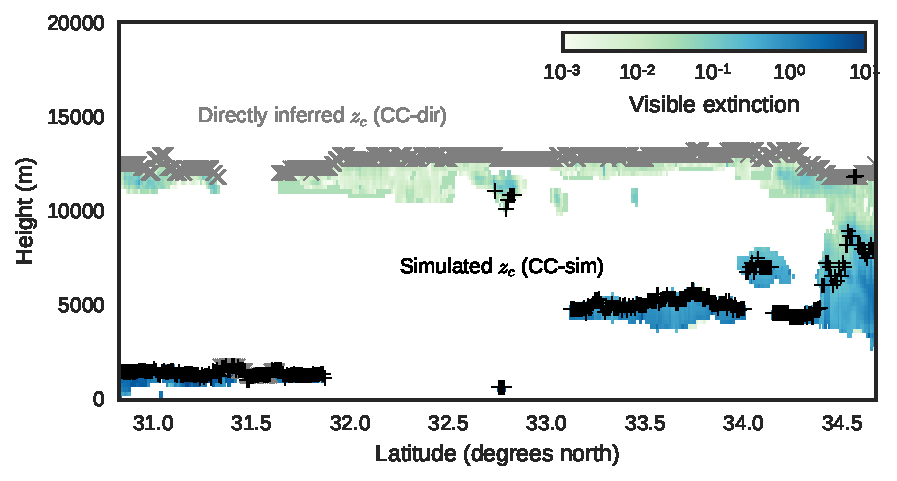
\includegraphics[width=\columnwidth]{graphics/misr_sim_example.pdf}
\caption{Profiles of visible extinction $d\tau$ and estimates of cloud top height $z_c$ for a short orbit segment.}
\label{misr_sim_example}
\end{figure}

The MISR simulator takes as a primary input a visible extinction profile (along with thermodynamic information) and outputs the cloud top height that MISR would likely retrieve for that profile. The estimates of the cloud top height ($z_c$) that MISR would likely retrieve (from a given input profile of visible extinction) are based on a number of simple rules, described in detail in \cite{marchand_and_ackerman_2010} (see Appendix A therein) and briefly summarized here in the context of Figure \ref{misr_sim_example}. The shading in Figure \ref{misr_sim_example} show an example of the combined CloudSat and CALIPSO (hereafter referred to as CC) cloud visible extinction retrieval for a short orbit section. The cloud top height estimated using two different methods is overlaid on the panel. First, cloud top height is estimated directly from the extinction profiles as the highest altitude for which the visible extinction is non-zero. This direct estimate of cloud top height (hereafter referred to as CC-dir) is indicated on the figure for each profile with a grey ``X''. Next, the simulated cloud top height (hereafter referred to as CC-sim) is diagnosed by passing the profiles of visible extinction to the MISR simulator. This estimate of cloud top height is indicated on the figure for each profile with a black ``+''. 

The example shown in Figure \ref{misr_sim_example} highlights several key aspects of how the MISR simulator works. For single-layer water clouds (which have large optical depth and high visible contrast), the MISR estimate of cloud top height is expected to be in good agreement with the ``true'' cloud top height, and thus CC-sim should agree well with CC-dir for these cases. For example, the extinction profile near 31.5 N shows a single low-level cloud layer with large optical depth, and the CC-dir and CC-sim estimates of cloud top height are similar. For multi-layer profiles where the upper cloud layer is sufficiently thin (nominally $\tau < 1$), MISR retrievals tend to effectively ``see through'' the upper-level, optically thin cloud, and retrieve the cloud top height of the lower cloud layer due to the fact that the lower cloud layer usually has more constrast in the scene and is preferentially picked up by the MISR pattern-matcher. The MISR simulator mimics this tendency (with again a nominal optical depth threshold for the upper layer of $\tau < 1$) and so the MISR simulator would return the cloud top height of the lower cloud layer in this case, even though the true cloud top height might be much higher in altitude, coinciding with the upper-level cloud. An example of this situation is seen in Figure \ref{misr_sim_example} near 33.5 N, where the CC-sim estimate returns the height of the lower cloud layer, but CC-dir returns the height of the upper cloud layer. For clouds with optically thicker ice-phase cloud tops, the MISR simulator penetrates down into the cloud layer to retrieve the cloud top height where the integrated optical depth reaches a nominal value of $\tau = 1$. In these cases (such as near 34.5 N in Figure \ref{misr_sim_example}), the simulated (CC-sim) cloud top height will also be lower than the true cloud top height, calculated directly by taking the highest level with non-zero extinction (CC-dir).

\begin{figure}
\centering
%\showthe\columnwidth
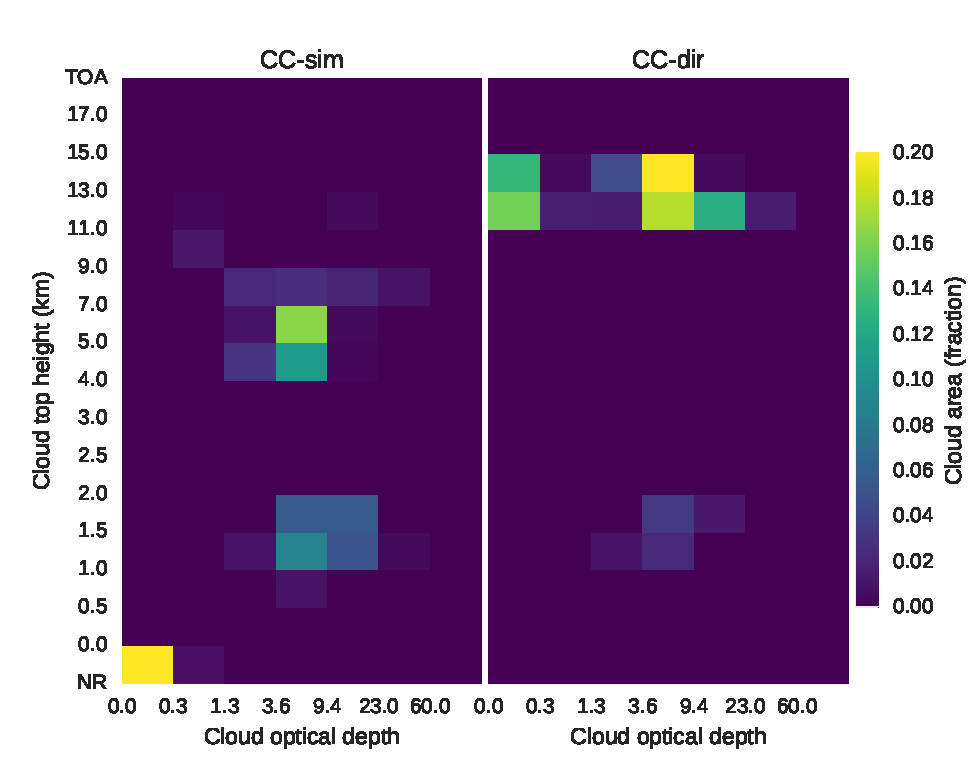
\includegraphics[width=\columnwidth]{graphics/misr_clmisr_example.pdf}
\caption{Joint histograms of cloud top height and optical depth for the example orbit segment shown in Figure \ref{misr_sim_example}.}
\label{misr_clmisr_example}
\end{figure}

Figure \ref{misr_clmisr_example} shows joint histograms of cloud top height and cloud optical depth for the example orbit segment shown above in Figure \ref{misr_sim_example}. The value of each element in the joint histogram is the relative frequency of occurrence of profiles within a certain cloud top height and optical depth range, and because each profile is assigned only one value of cloud top height and one value of cloud optical depth, the sum of the joint histogram values over all bins is equal to the total vertically projected cloud area. Likewise, the sum over all bins with cloud top height  $z_c \le 3$ km yields the low-topped cloud area, the sum over all bins with cloud top height $3 < z_c \le 7$ km yields the mid-topped cloud area, and the sum over all bins with cloud top height $z_c > 7$ km yields the high-topped cloud area. Taking the sum across the columns of the joint histogram yields the marginal histogram of cloud top height, and taking the sum across the rows yields the marginal histogram of cloud optical depth. 

The CC-sim joint histogram for this orbit has one low-topped mode with $0.5 < z_c < 2.0$ km (corresponding primarily to the low-level cloud at the far left of the top panel of \ref{misr_sim_example}) and a mid-topped mode with $4.0 < z_c < 9.0$ km (corresponding to the mid-level and deep cloud layers at the right of the top panel of the figure). There is also a large amount of cloud in the CC-sim joint histogram with $z_c < 0.0$ km. This cloud top height bin is reserved for profiles for which the MISR simulator determines that MISR would fail to retrieve a cloud top height. This often occurs for columns with very low optical depths. These no-retrieval cases correspond to the section of the example orbit in the top panel of the figure with a single-layer thin high-level cloud, between 32 and 33 N. The CC-dir joint histogram is dominated by a high-topped mode with $11.0 < z_c < 15.0$ km. There is also a much smaller low-topped mode with $1.0 < z_c < 2.0$ km, corresponding to the short section of the orbit with single-layered low-level cloud around 31.5 N.

The following section presents comparisons for two separate months (January and June 2008) of aggregated MISR, CC-sim, and CC-dir retrievals. 

\section{Comparisons between MISR-retrieved and MISR-simulated clouds}\label{misr_results}

Figure \ref{misr_cldmisr_maps_january} and Figure \ref{misr_cldmisr_maps_june} show maps of low-topped, mid-topped, high-topped, and total cloud cover from MISR retrievals and diagnosed from the CC visible extinction profiles with and without using the MISR simulator (CC-sim and CC-dir, respectively) for the months of January and June 2008. Data covers the domain with bounds -70N to 70N latitude and 100E to -70E longitude (this includes ocean surfaces beyond the Pacific Ocean, but we will refer to this domain as ``Pacific'' for convenience). Boxes are drawn around five climatically distinct regions that will be investigated more closely below: the North Pacific (35N to 60N; 160E to -140E), Hawaiian Trade Cumulus (15N to 35N; 160E to -140E), California Stratocumulus (15N to 35N; -140E to -110E), Tropical Western Pacific (-5N to 20N; 70E to 150E), and the South Pacific (-60N to -30N; -180E to -80E).

\begin{figure}
\centering
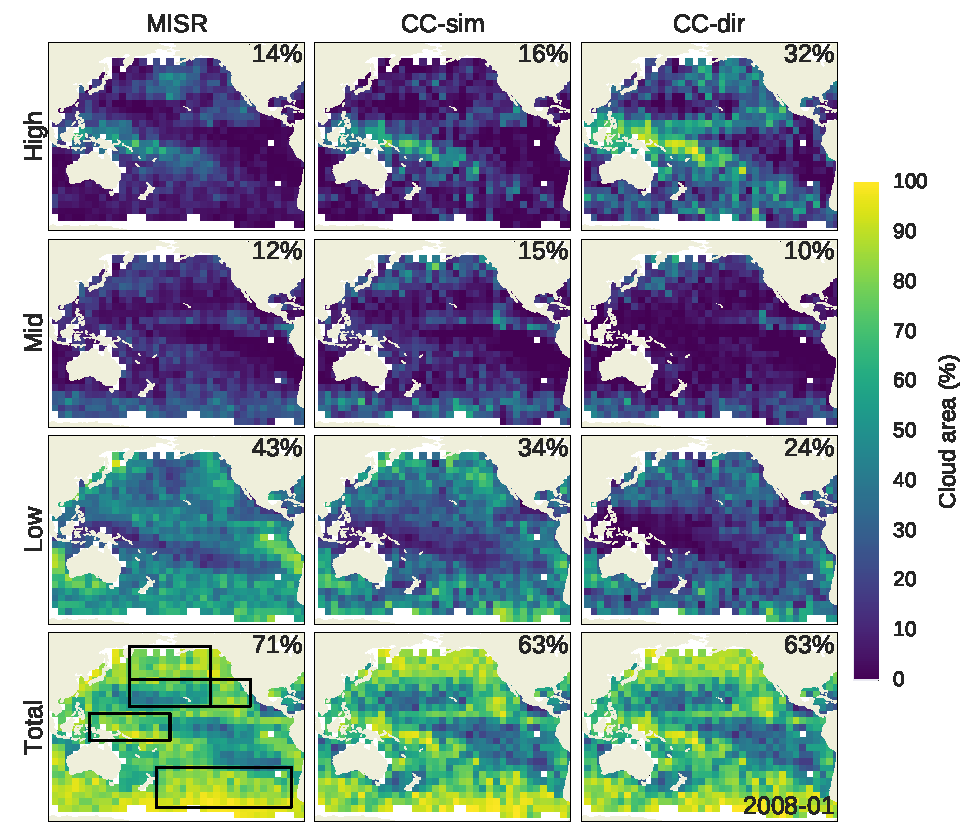
\includegraphics[width=\columnwidth]{graphics/misr_cldmisr_maps_2008-01.pdf}
\caption{Maps of cloud area by cloud type for January 2008 retrieved by MISR (left), diagnosed using the MISR simulator from extinction profiles retrieved from CloudSat/CALIPSO (middle), and diagnosed directly by taking the highest altitude with non-zero extinction from the CloudSat/CALIPSO extinction retrievals (right). Shown from top to bottom are total ($\tau > 0.3$), high-topped ($\tau > 0.3$; $z_c > 7$ km), mid-topped ($\tau > 0.3$; $3 < z_c < 7$ km), and low-topped ($\tau > 0.3$; $z_c < 3$ km) cloud area. Area-weighted domain averages are indicated in the upper-right corner of each panel.}
\label{misr_cldmisr_maps_january}
\end{figure}

\begin{figure}
\centering
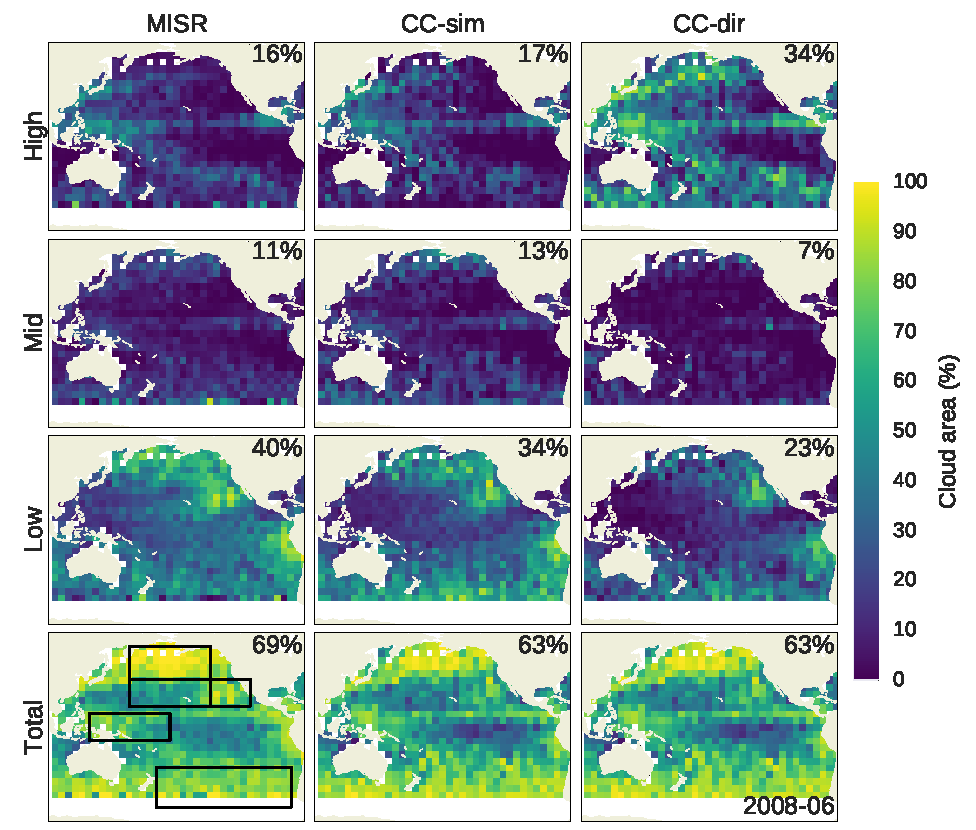
\includegraphics[width=\columnwidth]{graphics/misr_cldmisr_maps_2008-06.pdf}
\caption{Maps of cloud area by cloud type for June 2008 retrieved by MISR (left), diagnosed using the MISR simulator from extinction profiles retrieved from CloudSat/CALIPSO (middle), and diagnosed directly by taking the highest altitude with non-zero extinction from the CloudSat/CALIPSO extinction retrievals (right). Shown from top to bottom are total ($\tau > 0.3$), high-topped ($\tau > 0.3$; $z_c > 7$ km), mid-topped ($\tau > 0.3$; $3 < z_c < 7$ km), and low-topped ($\tau > 0.3$; $z_c < 3$ km) cloud area. Area-weighted domain averages are indicated in the upper-right corner of each panel.}
\label{misr_cldmisr_maps_june}
\end{figure}

These figures show that the cloud area by cloud type from the CC extinction retrieval using the MISR-simulator (CC-sim; middle panels) is broadly similar to the MISR-retrieved cloud area (left panels), especially as compared with the cloud area by cloud type diagnosed from the directly-inferred cloud top heights from the CC extinction retrieval (CC-dir; right panels). This indicates that (at least qualitatively) the MISR simulator is working as intended. Differences between CC-dir and CC-sim (and likewise between CC-dir and MISR) are especially large in the Tropical Warm Pool, North Pacific, and South Pacific regions, owing to the large occurrence of optically thin high-altitude cloud in these regions. Averaged over the entire region shown in the figure, the occurrence of high-topped clouds differs by only 2\% cloud area in January 2008 between CC-sim and MISR (16\% in CC-sim and 14\% in MISR retrievals), and by 1\% cloud area in June, and the occurrence of mid-topped clouds differs by only 2\% cloud cover in January (15\% in CC-sim and 13\% in the MISR retrievals), and by 3\% in June (14\% in CC-sim and 11\% in MISR retrievals). The largest difference between MISR and CC-sim is in low-topped cloud, where the low-topped cloud cover is smaller in CC-sim by 8\% in January and 6\% in June. However, much of this difference appears to be due to differences in low cloud detection between MISR and CC, rather than due to errors in the MISR simulator determination of cloud top height. This is supported by the estimates of total cloud cover, which also differ by 8\% and 6\% in January and June, respectively. This difference is due to differences in detection of low-level clouds by CC, which will be shown below.

\begin{figure}
\centering
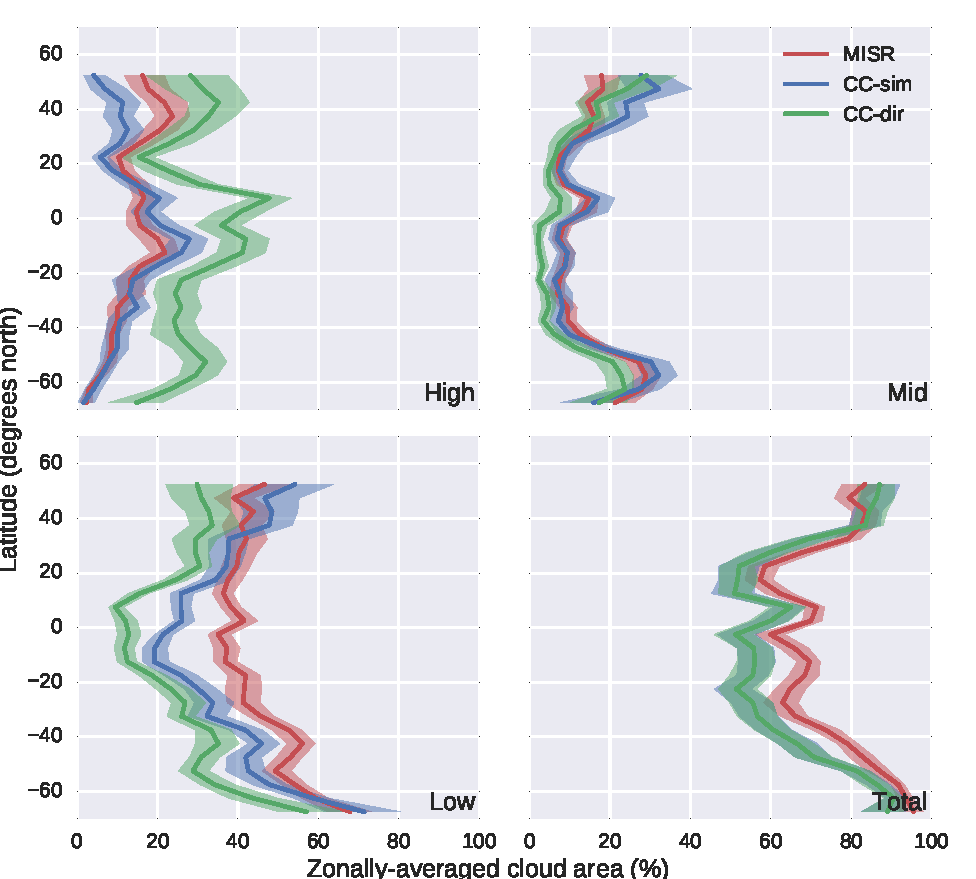
\includegraphics[width=\columnwidth]{graphics/misr_cldmisr_zonal_2008-01.pdf}
\caption{Zonally-averaged cloud area by cloud type from MISR-retrievals, MISR-simulated retrievals from CC-derived extinction profiles, and directly inferred cloud top heights from CC-derived extinction profiles for the month of January 2008. Shown are total, high-topped, mid-topped, and low-topped cloud area. Shading indicates the 95\% confidence interval obtained by bootstrap resampling the orbit-by-orbit zonal means.}
\label{misr_cldmisr_zonal_jan}
\end{figure}

\begin{figure}
\centering
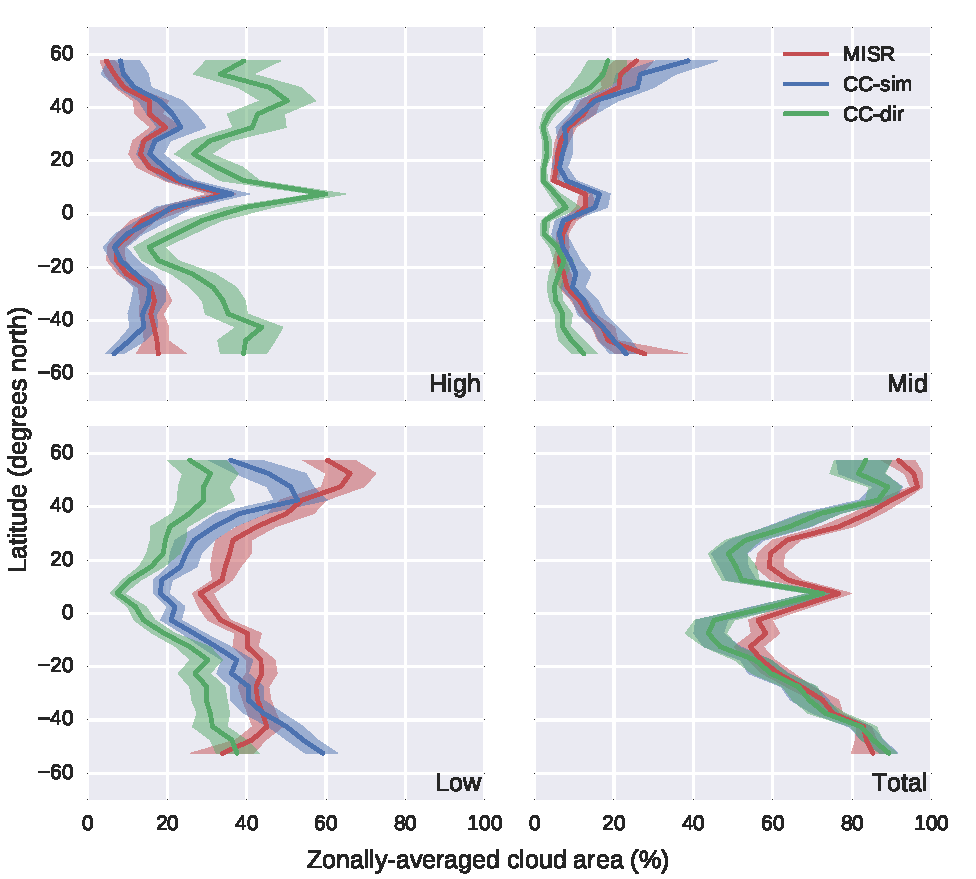
\includegraphics[width=\columnwidth]{graphics/misr_cldmisr_zonal_2008-06.pdf}
\caption{Zonally-averaged cloud area by cloud type from MISR-retrievals, MISR-simulated retrievals from CC-derived extinction profiles, and directly inferred cloud top heights from CC-derived extinction profiles for the month of June 2008. Shown are total, high-topped, mid-topped, and low-topped cloud area. Shading indicates the 95\% confidence interval obtained by bootstrap resampling the orbit-by-orbit zonal means.}
\label{misr_cldmisr_zonal_jun}
\end{figure}

The large impact the MISR simulator has on the estimate of cloud top height is clearly evident in the zonally-averaged cloud area by cloud top height, shown in Figures \ref{misr_cldmisr_zonal_jan} and \ref{misr_cldmisr_zonal_jun} for low, mid, and high-topped cloud cover (limited to the domain shown in Figures \ref{misr_cldmisr_maps_january} \ref{misr_cldmisr_maps_june}) for MISR, CC-sim, and CC-dir in January and June. Shaded regions show the 95\% confidence interval, based on 1000 bootstrap resamples of the orbit-by-orbit zonal means. A large fraction of the high-topped cloud detected by CC is not identified by the MISR stereo height retrieval, largely because it is optically thin (as will be shown later). The MISR simulator corrects for this in the CC retrieval, and the MISR-simulated high-topped cloud cover is in good agreement with the MISR retrievals except at northern mid-latitudes in January (30-60 N) and at high southern latitudes in June (south of 50 S) where differences are closer to 10\% and outside the range of sampling uncertainty indicated by the 95\% confidence interval shading. This may be due to several factors, including MISR detecting thinner cirrus in these regions (that is, clouds with an optical depth $\tau < 1$) because of contrast generated from long solar slant paths through the cirrus, or it may be due to limitations in the MISR stereo height algorithm. The MISR CTH-OD product uses the MISR stereo height retrieval with wind correction (the so-called ``best-winds'' retrieval) when cloud wind speed is successfully retrieved, and the stereo height ``without wind'' correction otherwise. The MISR stereo image matcher algorithm is in the process of being upgraded by the MISR Science Team, and the upgraded code (which will eventually lead to Version 7 of the MISR CTH-OD product) produces many more successful wind retrievals. Preliminary analysis of MISR CTH-OD Version 7 data indicates somewhat lower amounts of high-topped cloud in the North Pacific (closer to the CC-sim results) suggesting that the 10\% difference here may be at least partially due to incomplete wind speed correction, but a complete analysis of these errors is not possible until the new product is released.

The mid-topped MISR-simulated cloud area is also in very good agreement with the MISR retrievals, except for mid to high northern latitudes (north of 40 N in January and 50 N in June). Uncertainty bars are large at these latitudes because there is relatively little mid-topped cloud and relatively little ocean area at these latitudes. Nonetheless, it may well be that the MISR simulator is over-estimating the amount of MISR mid-topped cloud at these northern latitudes. The North Pacific is investigated in more detail later in this section.

There are large differences between MISR and CC-sim in the amount of both low-topped and total cloud. The occurrence of MISR low-topped cloud is much larger than CC-sim nearly everywhere except at high northern latitudes in January (north of 40 N) and at high southern latitudes in June (south of about 50 S) where CC-sim low-topped cloud exceeds MISR. This difference in low (and total cloud) area is likely due to differences in the instrument field-of-view or ``pixel size''. Because the field-of-view of satellite instruments can be partially filled by clouds, the fraction of satellite pixels containing some amount of cloud (the retrieved cloud fraction) will be larger than the true fractional area covered by clouds, and this difference generally increases as the satellite pixel size is increased \citep{digirolamo_and_davies_1997}. Of course, satellite retrievals do not perfectly identify partially cloud-filled pixels as cloudy, and there is a partial cancellation of errors which typically results in the satellite-retrieved cloud fraction being closer to the true fractional area covered by clouds than would be produced by a perfect cloud detector with the same resolution \citep{wielicki_and_parker_1992}. This resolution effect is particularly important for the small, broken clouds common in trade-wind cumulus in the subtropical dry zones, but applies to all broken boundary layer clouds \citep{zhao_and_digirolamo_2006, marchand_et_al_2010}. 

The effect that the detection of sub-pixel-sized clouds has on the retrievals is approximated here by creating a new joint radar-lidar cloud mask, modifying the thresholds used to identify cloudy versus clear profiles from the CloudSat and CALIPSO data. As described in Section \ref{cc_retrievals}, the CALIPSO data are mapped onto the coarser CloudSat grid in such a way that a combined retrieval (which uses the CloudSat grid) is only considered to have a lidar detection if 50\% of the CloudSat volume is filled by lidar detections, and so clouds smaller than the 1 km scale of the CloudSat grid are sometimes missed. The joint radar-lidar mask is then constructed by setting CloudSat bins as cloudy if either the CloudSat cloud mask identifies cloud (${\rm CPR\_Cloud\_mask} > 20$ in the 2B-GEOPROF product) or the lidar cloud fraction within that CloudSat bin is greater than 50\% (${\rm CloudFraction} > 50$ in the 2B-GEOPROF-LIDAR product). The sensitivity of the low-level cloud fraction (the fraction of profiles with \emph{any} cloud below 3 km, not just profiles with cloud \emph{tops} below 3 km as reported by MISR) to the lidar cloud fraction threshold is quantified here by adjusting the lidar cloud fraction threshold for considering cloud to 0\% and 10\% and comparing the resulting low-level cloud fraction to that obtained using the 50\% threshold.

\begin{figure}
\centering
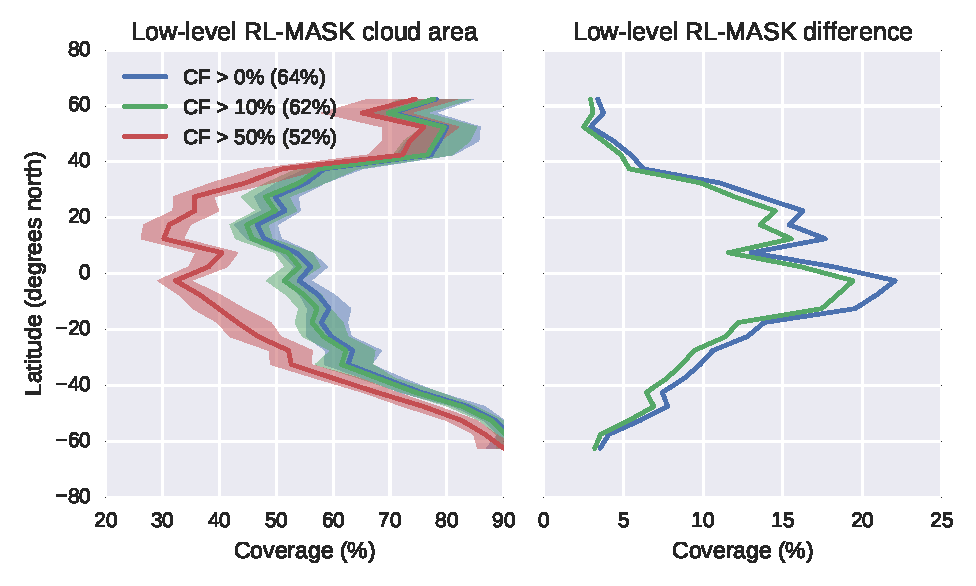
\includegraphics[width=\columnwidth]{graphics/misr_rlmask_test.pdf}
\caption{Joint radar-lidar low-level cloud mask from 2B-GEOPROF and 2B-GEOPROF-LIDAR for different lidar cloud fraction thresholds over the Pacific domain. Height bins are considered "cloudy" if the radar cloud mask (CPR\_Cloud\_mask in 2B-GEOPROF) has a value greater than 20, or if the lidar cloud fraction (CloudFraction in 2B-GEOPROF-LIDAR) is greater than the selected threshold value (indicicated in the legend). Plotted are the zonally averaged fraction of profiles with any cloudy height bins below 3 km (left), and differences relative to the default threshold of 50\% (right). Numbers in parentheses in the legend indicate the average over the entire (Pacific) domain.}
\label{misr_rlmask_test}
\end{figure}

Figure \ref{misr_rlmask_test} shows the zonally-averaged low-level cloud fraction from the joint radar-lidar mask for the same domain used in the MISR analysis (ice-free ocean between -70 to 70 N and between 100 E and -70 E) using the three threshold values for lidar cloud fraction, as well as the differences relative to using the 50\% cloud fraction threshold. The domain-averaged difference in low-level cloud area is 12\%, and differences in the zonally-averaged low-level cloud area are as high as 22\% in the tropical Pacific. Differences are mch smaller at higher latitudes, and differences in the north Pacific are generally less than 5\% cloud area. Nonetheless, this analysis shows a very large sensitivity to the fraction of lidar-detected clouds kept, and suggests a large resolution dependence on the low-level (and total) cloud area. The resolution-driven increase in MISR-retrieved low-topped cloud due to this partially filled pixel problem is likely to be of a similar magnitude, and thus the large differences identified in Figures \ref{misr_cldmisr_zonal_jan} and \ref{misr_cldmisr_zonal_jun} for total and low-topped cloud throughout the low latitudes is very likely due primarily to an overestimation by MISR of the cloud area. Sensitivities to this detection threshold are much lower in the high latitudes, and the close agreement in total cloud fraction between MISR and CC at high-latitudes in the winter hemisphere demonstrated in Figures \ref{misr_cldmisr_zonal_jan} and \ref{misr_cldmisr_zonal_jun} demonstrates the more horizontally continuous (or wider-spread) nature of low clouds during the winter season at these latitudes, especially in the southern hemisphere.

\begin{figure}
\centering
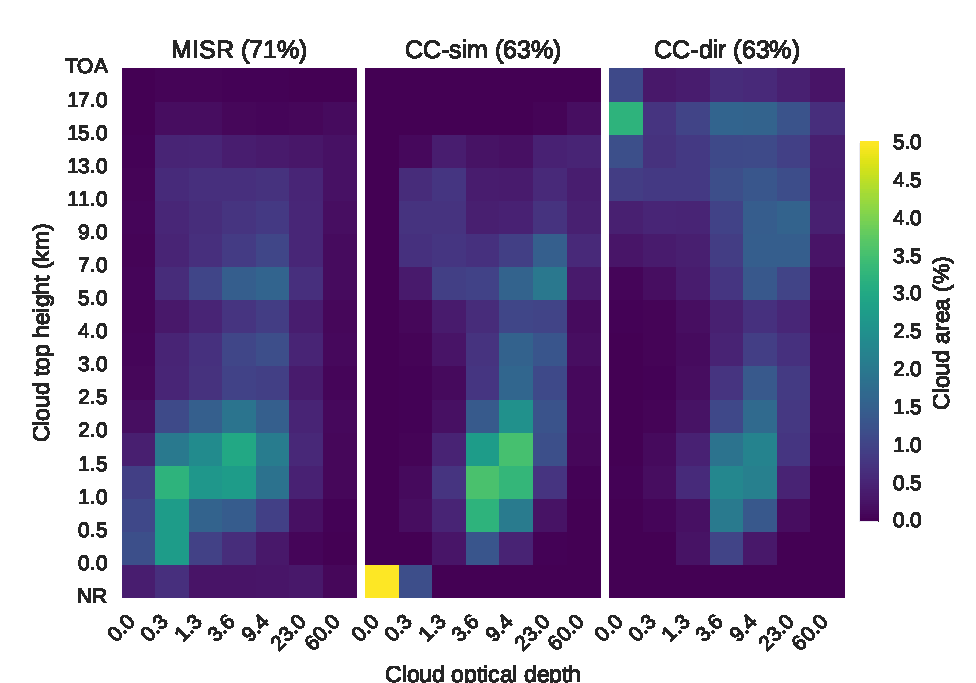
\includegraphics[width=\columnwidth]{graphics/misr_clmisr_Pacific_2008-01.pdf}
\caption{Joint histograms of cloud top height and cloud optical depth for January 2008.}
\label{misr_cthtau_Pacific_january}
\end{figure}

\begin{figure}
\centering
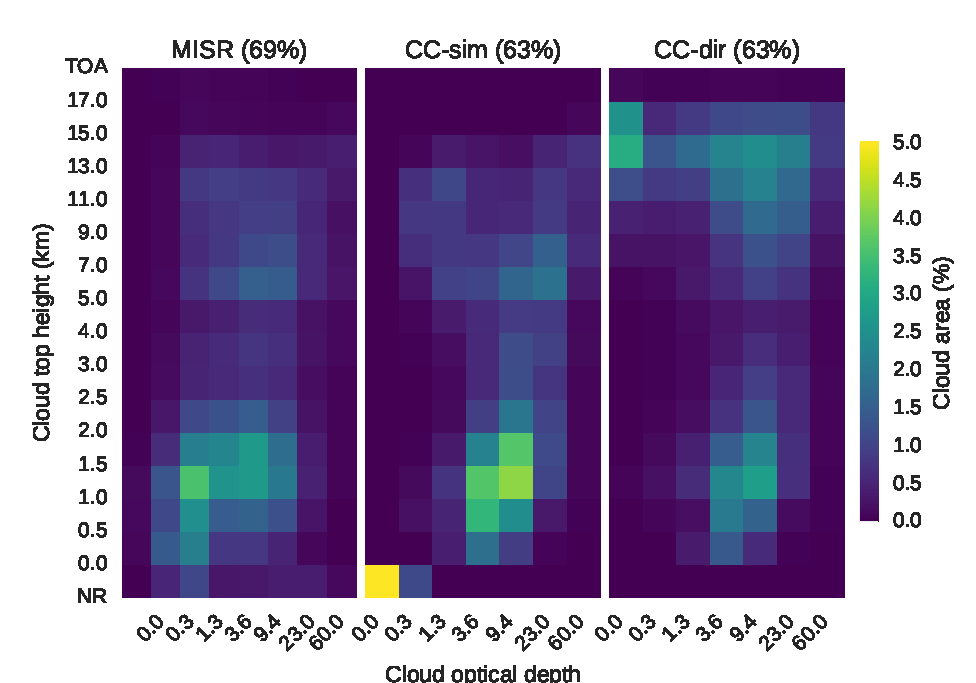
\includegraphics[width=\columnwidth]{graphics/misr_clmisr_Pacific_2008-06.pdf}
\caption{Joint histograms of cloud top height and cloud optical depth for June 2008.}
\label{misr_cthtau_Pacific_june}
\end{figure}

Cloud 3D structure and partially-filled satellite pixels are also well-known to affect imager retrievals of cloud optical depth, which are based on 1D radiative transfer and effectively assume homogenous plane parallel clouds \citep{yang_and_digirolamo_2008, evans_et_al_2008}. Figure \ref{misr_cthtau_Pacific_january} and Figure \ref{misr_cthtau_Pacific_june} show the cloud top height and optical depth joint histograms for the entire analysis region for January and June 2008, respectively. The MISR retrieved joint histograms have a low-topped ($z_c < 3$ km) maximum at low to moderate optical depths ($\tau < 23$), and a mid to high-topped maximum ($5 < z_c < 13$ km) at moderate optical depths ($3.6 < \tau < 23$). The CC-sim joint histograms have a similar bimodal structure, but with considerably smaller amounts of cloud with low optical depth ($\tau < 3.6$) and large amounts of cloud with high optical depth ($\tau > 9.4$), consistent with expectations for errors due to partially filled pixels and reliance on 1D radiative transfer \citep{marchand_et_al_2010}. The large differences in the CC-dir histograms again illustrate the importance of accounting for the effects of multi-layered and optically thin cloud profiles in the  distribution.

\begin{figure}
\centering
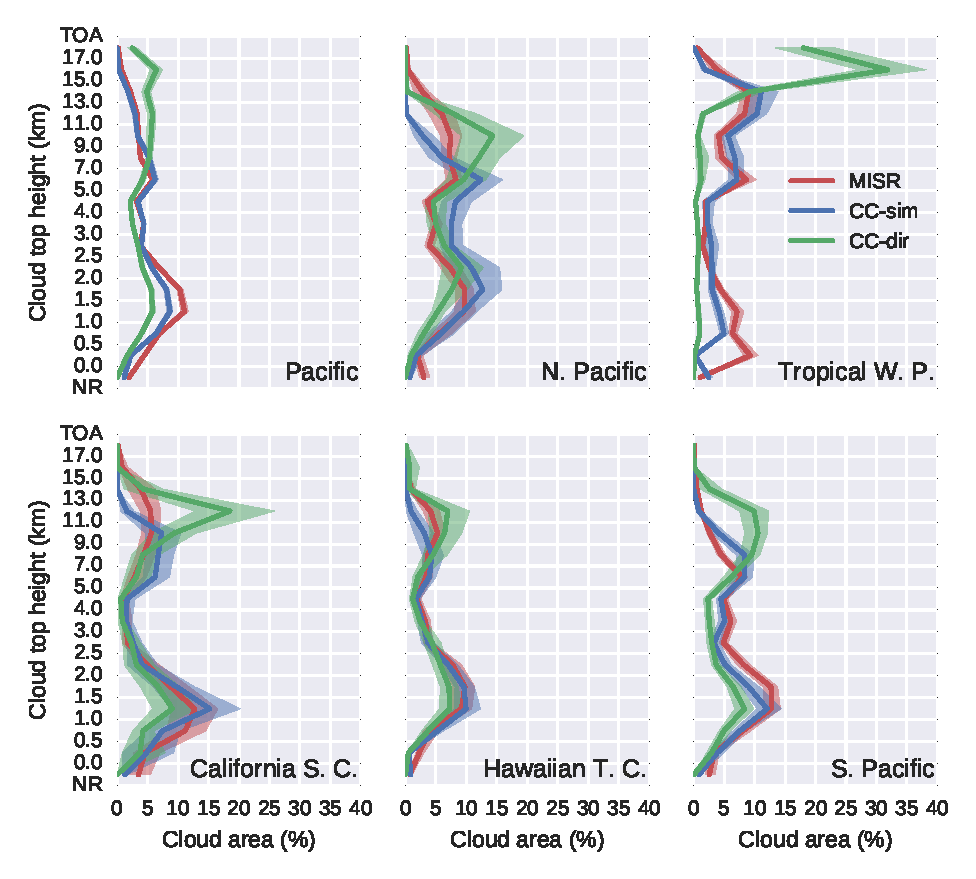
\includegraphics[width=\columnwidth]{graphics/misr_cth_2008-01.pdf}
\caption{Histograms of cloud top height for January.}
\label{misr_cth_region_january}
\end{figure}

\begin{figure}
\centering
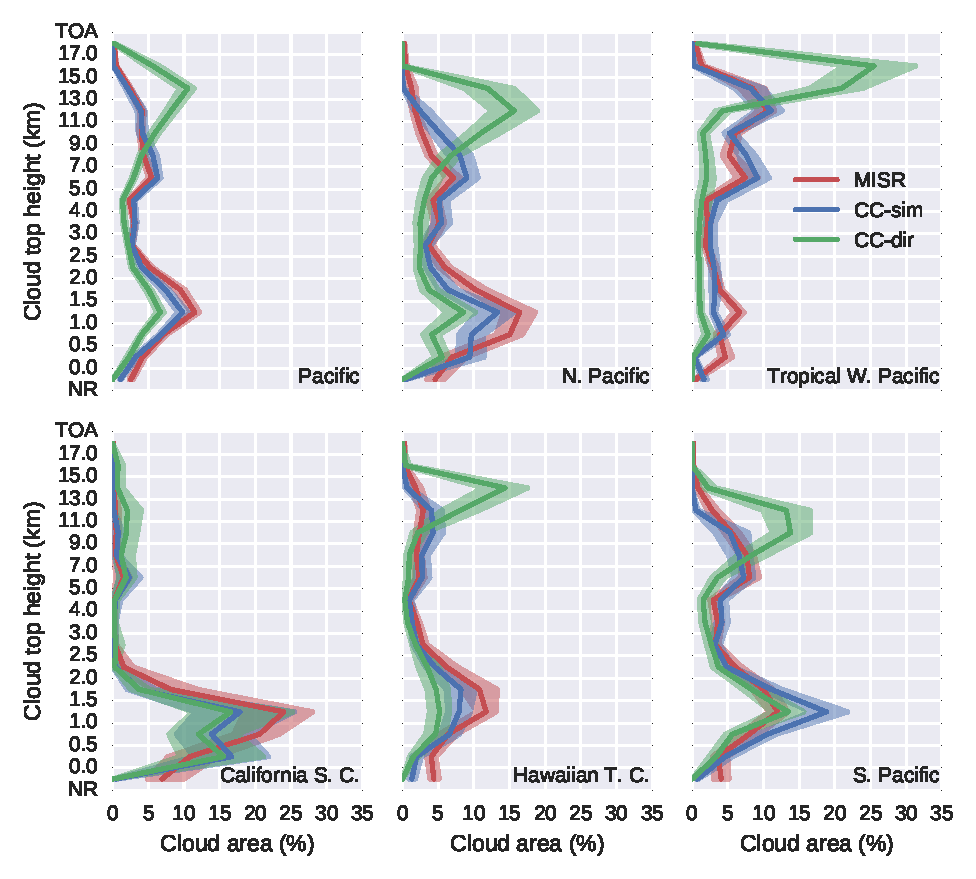
\includegraphics[width=\columnwidth]{graphics/misr_cth_2008-06.pdf}
\caption{Histograms of cloud top height for June.}
\label{misr_cth_region_june}
\end{figure}

Figures \ref{misr_cth_region_january} and \ref{misr_cth_region_june} show marginal histograms of cloud top height ($z_c$) for each of the regions outlined in Figure \ref{misr_cldmisr_maps_january} and \ref{misr_cldmisr_maps_june}. Regionally averaged cloud area by cloud type is summarized for each of these regions in Tables \ref{misr_cldmisr_table_january} and \ref{misr_cldmisr_table_june} for January and June, respectively. The tables show the regionally averaged cloud area by cloud type for the MISR and CC-sim retrievals, the difference between CC-sim and MISR, and the significance level of the differences calculated using a Welch's (two-sample, unequal size, unequal variance) Student $t$-test, treating each orbit as an independent sample. With the exception of the California Stratus region, the CC-dir results show large amounts of high-topped clouds in both January and June. Most of this high-topped cloud is optically thin, and the MISR simulator does a reasonable job matching the MISR retrievals. The good agreement between MISR and CC-sim mid and high-topped cloud is also evident in Tables \ref{misr_cldmisr_table_january} and \ref{misr_cldmisr_table_june}, which show that the more broadly defined mid and high-topped categories are in even better agreement than the profiles of cloud top height shown in Figures \ref{misr_cth_region_january} and \ref{misr_cth_region_june}, with differences generally less than 5\%, and the only statistically significant differences being in the North Pacific [check this]. As discussed earlier, the differences in the North Pacific in January may reflect biases due to incomplete wind correction in the MISR CTH-OD V6 product. Differences in the other regions are much smaller than those in the North Pacific (typically less than 5\% cloud area) and are generally not statistically significant with respect to sampling.

As discussed previously, low-topped differences can be large even when using the simulator to correct for the effects of thin high-topped cloud on the retrievals due to differences in low-level cloud detection between the different observing platforms. This is especially true in the California Stratocumulus, Hawaiian Trade Cumulus, and North Pacific regions (in the NH summer) due to field-of-view issues, but these regions also have large variability in low-topped cloud amount, as indicated by the large sampling uncertainties for low-topped cloud bins in these regions. Table \ref{misr_cldmisr_table_june} shows that low-topped cloud differences in June are largest in the California SC region, where CC-sim low-topped cloud amount (using the 50\% lidar cloud fraction threshold as discussed above in the context of Figure \ref{misr_rlmask_test}) is lower than MISR by 15\% cloud area. While this region is well known for its extensive low cloud, this cloud often displays considerable spatial structure and broken cloudiness. \cite{klein_and_hartmann_1993} found using ship-based observer reports (following \cite{warren_et_al_1986, warren_et_al_1988}) that low (stratus) cloud cover in this region can exceed 60\% cloud area in summer months, reaching a peak value of 67\%. This is consistent with the low-topped cloud cover found here from MISR retrievals. Low-topped cloud amounts are lower in this region in January, and the differences are much smaller and are not statistically significant with respect to sampling.

\begin{table}
\centering
\begin{tabular}{lcccccc}
\hline\hline
Region & Cloud type &  MISR & CC-sim &  Diff & p-value & Significance \\ \hline
   Pacific &       High &  13.2 &  13.0 &  -0.2 & 0.989 &       \\
           &        Mid &  13.7 &  14.9 &   1.1 & 0.512 &       \\
           &        Low &  44.4 &  36.4 &  -8.0 & 0.000 &    ** \\
           &      Total &  73.3 &  65.3 &  -8.0 & 0.000 &    ** \\
\hline
N. Pacific &       High &  23.5 &   9.6 & -13.9 & 0.000 &    ** \\
           &        Mid &  16.5 &  26.9 &  10.3 & 0.001 &    ** \\
           &        Low &  38.3 &  48.3 &  10.0 & 0.015 &     * \\
           &      Total &  81.5 &  85.6 &   4.1 & 0.336 &       \\
\hline
Tropical W. P. &       High &  29.6 &  37.2 &   7.6 & 0.047 &     * \\
           &        Mid &  12.3 &  11.2 &  -1.0 & 0.468 &       \\
           &        Low &  32.9 &  17.5 & -15.4 & 0.000 &    ** \\
           &      Total &  75.5 &  68.5 &  -7.0 & 0.018 &     * \\
\hline
California S. C. &       High &  20.9 &  15.6 &  -5.4 & 0.924 &       \\
           &        Mid &   5.3 &   9.4 &   4.0 & 0.072 &       \\
           &        Low &  44.3 &  43.4 &  -0.8 & 0.989 &       \\
           &      Total &  74.3 &  69.7 &  -4.5 & 0.846 &       \\
\hline
Hawaiian T. C. &       High &  14.8 &   8.3 &  -6.5 & 0.005 &    ** \\
           &        Mid &   8.1 &   8.7 &   0.6 & 0.979 &       \\
           &        Low &  36.5 &  35.1 &  -1.3 & 0.943 &       \\
           &      Total &  60.0 &  52.9 &  -7.1 & 0.006 &    ** \\
\hline
S. Pacific &       High &   9.0 &  11.6 &   2.6 & 0.066 &       \\
           &        Mid &  19.0 &  18.8 &  -0.2 & 0.288 &       \\
           &        Low &  50.8 &  42.1 &  -8.7 & 0.005 &    ** \\
           &      Total &  81.5 &  73.4 &  -8.0 & 0.000 &    ** \\
\hline
\end{tabular}

\caption{Regional mean cloud area by cloud top height for January 2008.}
\label{misr_cldmisr_table_january}
\end{table}

\begin{table}
\centering
\begin{tabular}{lcccccc}
\hline\hline
Region & Cloud type &  MISR & CC-sim &  Diff & p-value & Significance \\ \hline
   Pacific &       High &  15.5 &  15.7 &   0.1 & 0.532 &       \\
           &        Mid &  10.7 &  12.7 &   2.0 & 0.000 &    ** \\
           &        Low &  41.0 &  35.3 &  -5.7 & 0.000 &    ** \\
           &      Total &  69.8 &  64.8 &  -5.1 & 0.000 &    ** \\
\hline
N. Pacific &       High &  10.8 &  15.6 &   4.8 & 0.045 &     * \\
           &        Mid &  19.0 &  23.6 &   4.6 & 0.004 &    ** \\
           &        Low &  60.6 &  48.6 & -12.0 & 0.000 &    ** \\
           &      Total &  94.2 &  88.2 &  -6.0 & 0.001 &    ** \\
\hline
Tropical W. P. &       High &  32.2 &  32.1 &  -0.1 & 0.567 &       \\
           &        Mid &  11.7 &  14.6 &   2.9 & 0.097 &       \\
           &        Low &  24.6 &  16.7 &  -7.8 & 0.003 &    ** \\
           &      Total &  69.0 &  65.0 &  -3.9 & 0.242 &       \\
\hline
California S. C. &       High &   1.8 &   1.7 &  -0.0 & 0.689 &       \\
           &        Mid &   2.0 &   2.6 &   0.6 & 0.418 &       \\
           &        Low &  66.2 &  51.7 & -14.5 & 0.024 &     * \\
           &      Total &  76.8 &  56.5 & -20.3 & 0.001 &    ** \\
\hline
Hawaiian T. C. &       High &   9.8 &  12.3 &   2.5 & 0.727 &       \\
           &        Mid &   5.4 &   5.3 &  -0.1 & 0.888 &       \\
           &        Low &  42.0 &  31.3 & -10.6 & 0.000 &    ** \\
           &      Total &  61.6 &  50.2 & -11.4 & 0.000 &    ** \\
\hline
S. Pacific &       High &  16.4 &  11.9 &  -4.5 & 0.049 &     * \\
           &        Mid &  14.6 &  16.0 &   1.4 & 0.627 &       \\
           &        Low &  43.7 &  52.9 &   9.1 & 0.000 &    ** \\
           &      Total &  78.8 &  81.5 &   2.7 & 0.024 &     * \\
\hline
\end{tabular}

\caption{Regional mean cloud area by cloud top height for June 2008.}
\label{misr_cldmisr_table_june}
\end{table}

\section{Diurnal variations in cloud cover} \label{misr_diurnal}
Some of differences discussed in the previous section between MISR and CC-sim may arise due to diurnal differences in the true cloud height or cloud area since MISR overpass times (on the Terra platform; 10:30 AM local equatorial crossing time) are roughly three hours different (at the equator) than CloudSat and CALIPSO (in the A-train constellation; 3:30 PM local equatorial crossing time). There are MODIS instruments on both the Terra and Aqua (which is also in the A-train constellation) satellites, and in this section retrievals from the MODIS Terra and Aqua sensors are compared in order to provide a measure of the differences in cloud properties between the two overpass times. Of course, some of the difference between MODIS Terra and Aqua cloud cover may be due to differences in the sensors and their performance, but these are thought to be small \citep{king_et_al_2013}. \cite{king_et_al_2013} use this strategy to evaluate diurnal differences in cloud cover by comparing 12 years of MODIS Terra (MOD35) and 9 years of MODIS Aqua (MYD35) cloud masks. They find cloud cover over ocean is in general slightly greater in the Terra retrievals than in those from Aqua, suggesting a decrease in cloud cover from the morning to afternoon overpass. \cite{king_et_al_2013} show that differences between Terra and Aqua are largest in regions dominated by coastal marine stratocumulus, and Terra to Aqua differences approach 20\% cloud cover in the Peruvian and Angolan stratocumulus regions from September to February. However, zonal average differences are much smaller, and global averages agree to within 5\% cloud cover between Terra and Aqua. \cite{meskhidze_et_al_2009} similarly look at differences between Aqua and Terra liquid cloud amount and likewise find a reduction in both cloud amount and cloud optical depth in stratocumulus (and trade wind cumulus) regions between the morning and afternoon overpasses, with differences in the Peruvian and South African stratocumulus on the order of 20\% cloud cover during the months of December to February. These results are consistent with the diurnal cycle in cloud amount expected from both modeling studies and field campaign studies, which show that cloud cover reaches a maximum in the early morning and decreases throughout the day, reaching a minimum in the early afternoon \citep{bretherton_et_al_2004}.

Terra to Aqua differences reported in \cite{king_et_al_2013} and \cite{meskhidze_et_al_2009} for the regions studied here are more modest. \cite{king_et_al_2013} show differences in June-July-August total cloud cover for the California Stratus region are about 10\%, and differences in the North Pacific for these months is much less than 5\%. Nonetheless, these differences in cloud cover are non-trivial, and are of the correct sign to explain at least some of the differences between MISR and CC-sim low cloud cover shown in the previous section.

\begin{figure}
\centering
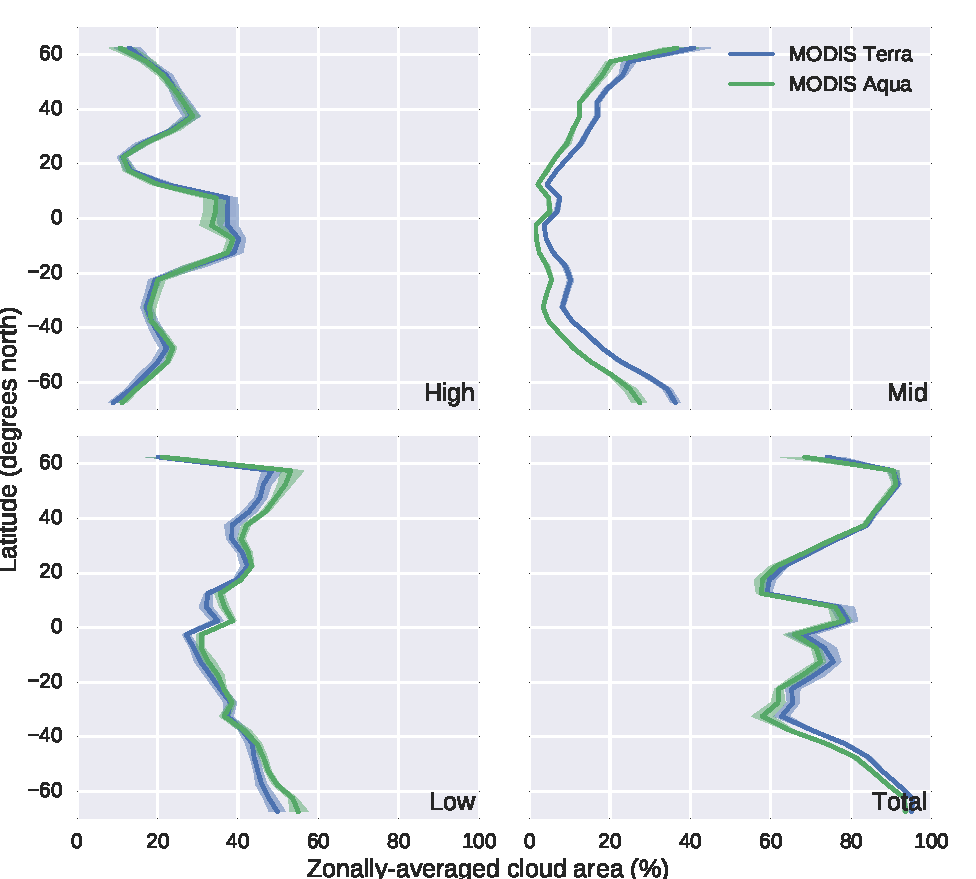
\includegraphics[width=\columnwidth]{graphics/misr_cldmodis_zonal_2008-01.pdf}
\caption{January climatology of zonally-averaged cloud area from MODIS Terra and Aqua over the Pacific domain. Shading indicates 95\% confidence interval obtained by bootstrap resampling individual monthly-means.}
\label{misr_cldmodis_zonal_january}
\end{figure}

\begin{figure}
\centering
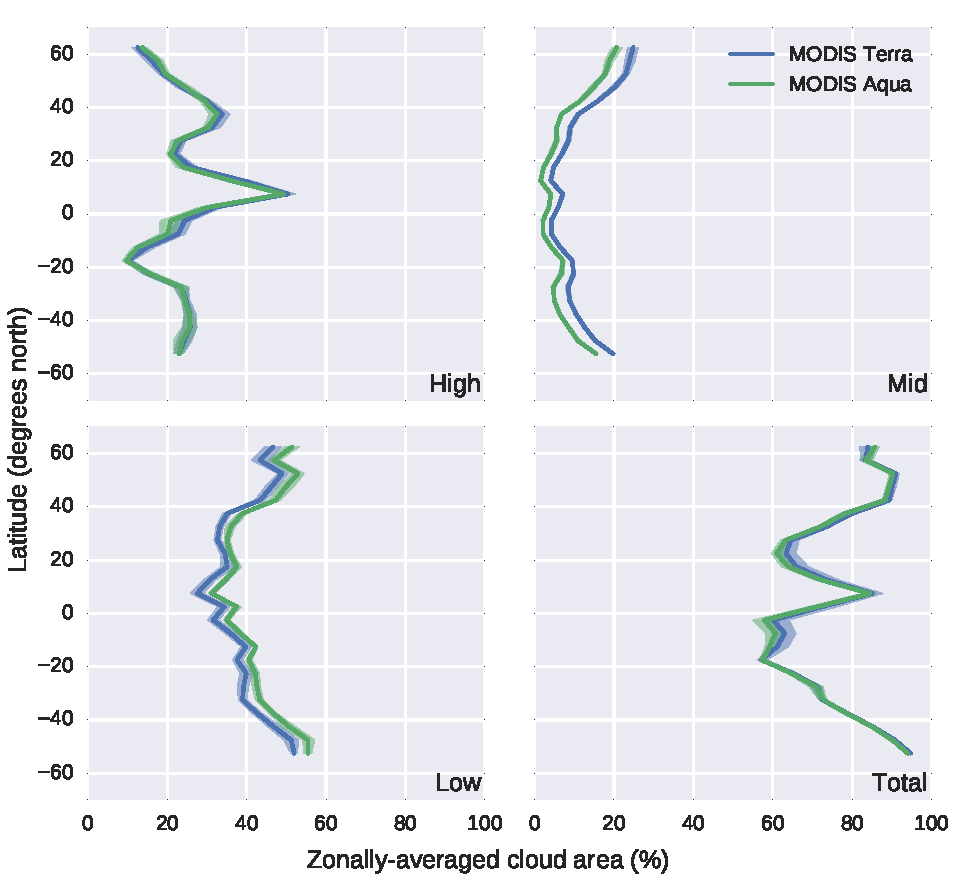
\includegraphics[width=\columnwidth]{graphics/misr_cldmodis_zonal_2008-06.pdf}
\caption{June climatology of zonally-averaged cloud area from MODIS Terra and Aqua over the Pacific domain. Shading indicates 95\% confidence interval obtained by bootstrap resampling individual monthly-means.}
\label{misr_cldmodis_zonal_june}
\end{figure}

Figures \ref{misr_cldmodis_zonal_january} and \ref{misr_cldmodis_zonal_june} show zonally-averaged MODIS total, high-topped (cloud top pressure $p_c < 440$ hPa), mid-topped ($440 < p_c < 680$ hPa) and low-topped ($p_c > 680$ hPa) cloud area using data from 12 years (2003 to 2014) and restricted to ocean areas in the Pacific analysis region shown in Figures \ref{misr_cldmisr_maps_january} and \ref{misr_cldmisr_maps_june} for the months of January and June, respectively. The zonal mean total cloud cover (bottom right panels) are nearly indistinguishable between the Terra and Aqua retrievals (less than 2\% cloud cover difference throughout most of the domain), and the small differences that do exist in total cloud cover are not statistically significant with respect to sampling. There are, however, noticeable differences between the Terra and Aqua low and mid-topped cloud cover, with the Terra mid-topped cloud cover being larger than Aqua. The differences are significant in the sense that they are larger than could be explained by sampling (as represented by the error bars showing the 95\% confidence interval). The differences in mid-topped and low-topped zonal mean cloud area are a bit less than 6\% and 5\%, respectively, but this is comparable to the difference between MISR retrieved and MISR-simulated mid-topped cloud amount found in Section \ref{misr_results}, which suggests this difference may be near the limit of agreement that one should expect given our evaluation approach.

% Section
\section{Summary and discussion}
\label{misr_summary}
Satellite instrument simulators are used increasingly more in model evaluation studies to account for known features, limitations, or errors in individual satellite retrievals. However, as recognized by \cite{pincus_et_al_2012} and \cite{mace_et_al_2011}, not all such errors or ambiguities have been (or likely can be) removed by this approach, and critical evaluation of the simulators themselves is of the utmost importance if the simulator framework is to be used to quantify biases between satellite-retrieved and model-simulated cloud properties. This chapter has presented an evaluation of the MISR simulator by comparing MISR retrievals to MISR-simulated retrievals based on extinction profiles derived from a combination of CloudSat, CALIPSO, and MODIS observations. 

The results in this chapter show that mid and high-topped cloud cover is in good agreement between MISR and MISR-simulated retrievals from CC. Global, zonal and regionally-averaged mid and high-topped cloud cover differences are typically small (on the order of 5\% cloud cover or less) and not statistically significant with respect to sampling. Marginal histograms of cloud top height capture the main features of the cloud top height distribution, including the altitude of peaks in cloud top height.  The most notable exception to this is high-topped cloud amounts in the winter hemisphere poleward of 50 degrees, where differences are closer to 10\% cloud area.  It is expected that this problem will be at least reduced in the next release (Version 7) of the MISR CTH-OD dataset. An analysis of Version 7 results is not yet possible and will be the focus of future research for the MISR Science Team.

Uncertainties in low-topped cloud remain large in this comparison, with differences between MISR and CC-sim between 5 and 15\% cloud area for the specific regions studied here, and with differences in MISR and CC-sim zonal means often exceeding 10\% cloud area. This is likely due to differences in detection of partially filled cloudy pixels (sensor field-of-views) between MISR and CC, rather than being indicative of a problem with the MISR simulator. Nonetheless, these errors need to be considered when comparing model-simulated cloud area with MISR-retrieved cloud area, as the MISR-retrieved cloud area is likely biased high in regions occupied by small broken boundary-layer clouds. This bias is of the correct sign to explain at least some of the ubiquitous ``biases'' in low-level cloud amount in current global climate models as compared with retrievals from MISR, ISCCP, and MODIS, as will be shown in Chapter \ref{cmip5_chapter}, suggesting that at least some of these differences are more appropriately attributed to systematic biases in our retrievals. This is an area of on-going research in the remote sensing community [citations needed].

Differences in the full cloud top height and optical depth joint histograms for the whole domain had an absolute error of 4\% or less for any particular cloud-type ($z_c$-$\tau$ bin). For comparison, M2011 looked at coincident ISCCP and ISCCP-simulated retrievals derived from ARM SGP data, and report absolute errors in the coarsened 9-bin ISCCP  histograms that are typically under 4\% as well, but can be as high as 8\% for low, optically thick clouds (see Figure 4 in M2011). Much of the difference between the MISR-retrieved (or ISCCP-retrieved) joint histogram and that obtained from the simulator (using CC retrievals as input) is due to a systematic trend toward higher values of cloud optical depth in the CC retrieval than in MISR (or ISCCP) retrievals. While for low clouds the effect of sensor resolution and 3D effects on visible radiances may explain much or most of the difference, the situation is less clear for high and mid-level clouds, which tend to occur on larger horizontal scales. While 3D effects may still be significant for high and mid-level clouds, other factors may also be important. In particular, retrievals of optical depth from radar and lidar may be prone to overestimate optical depth for a variety of factors including the strong sensitivity of radar to precipitating particles (which makes retrieval of small or non-precipitating particles that usually dominate the visible-extinction difficult and uncertain), especially at temperatures where both ice and water condensate may exists.

[TODO: add a strong conclusion here]
% End of chapter
